\chapter{GCN e baseline}
\label{ch:forecasting-models}

\section{Dal percettrone al layer su grafo}
\label{sec:from-perceptron-to-graph-layer}

Il \Cref{ch:graph-laplacian-theory} ha fornito gli strumenti necessari per descrivere un grafo pesato e quantificarne la connettività tramite il Laplaciano, utilizzati ora per definire un modello che apprende dai dati. Il punto di partenza è il modello neurale più semplice, il percettrone multistrato (\emph{multilayer perceptron}, MLP), che rappresenta l'input come un vettore $h^{(0)}\in\mathbb{R}^{F_0}$ e lo trasforma applicando in sequenza $L$ strati della forma
\begin{equation}
\label{eq:mlp-layer}
h^{(l+1)} = \sigma\!\left(W^{(l)}h^{(l)} + b^{(l)}\right),
\end{equation}
ove $h^{(l)}$ è la rappresentazione del sistema allo strato $l$, $W^{(l)}\in\mathbb{R}^{F_{l+1}\times F_l}$ e $b^{(l)}\in\mathbb{R}^{F_{l+1}}$ sono parametri appresi\footnote{Nel \Cref{ch:graph-laplacian-theory} il simbolo $W$ denota la matrice dei pesi del grafo. $W^{(l)}$ denota invece la matrice dei parametri appresi dallo strato $l$ nelle reti neurali. Nel seguito la distinzione è affidata all'apice: $W$ resta la matrice dei pesi del grafo, $W^{(l)}$ è sempre una matrice di parametri.} e $\sigma$ è una funzione non lineare applicata componente per componente. La non linearità è essenziale: componendo strati puramente lineari si otterrebbe ancora una trasformazione lineare e la profondità non aggiungerebbe alcuna capacità espressiva~\cite{goodfellow2016deep}.

I parametri si stimano minimizzando una funzione di costo $C$ tramite discesa del gradiente, che sposta ciascun peso nella direzione che riduce maggiormente tale costo. Il gradiente $\partial C/\partial W^{(l)}$ misura la sensibilità della funzione $C$ ad una variazione di ogni peso e si calcola tramite backpropagation~\cite{rumelhart1986learning}, l'applicazione sistematica della regola della catena che percorre all'indietro il grafo computazionale definito dalla composizione degli $L$ strati.

Poiché, per l'equazione~\eqref{eq:mlp-layer}, $h^{(l+1)}$ dipende da $h^{(l)}$ solo attraverso lo strato $l+1$, la regola della catena esprime il gradiente rispetto al peso $w^{(l)}_{ij}$ in funzione di quello rispetto a $h^{(l+1)}$ e dello jacobiano dello strato stesso, nella forma esplicita
\begin{equation}
\label{eq:backprop-weight-gradient}
\frac{\partial C}{\partial w^{(l)}_{ij}} = \frac{\partial C}{\partial h^{(l+1)}_i} \cdot \sigma'\!\left(z^{(l+1)}_i\right) \cdot h^{(l)}_j, \qquad z^{(l+1)} = W^{(l)}h^{(l)} + b^{(l)}.
\end{equation}
La backpropagation sfrutta questa struttura calcolando il gradiente a ritroso. Partendo dal gradiente rispetto a $h^{(L)}$, ottenuto direttamente dalla funzione di costo, ogni gradiente rispetto a $h^{(l+1)}$ già noto viene riutilizzato sia per il calcolo del gradiente rispetto a $W^{(l)}$, sia per quello rispetto a $h^{(l)}$. Si prosegue verso gli strati precedenti senza mai ricalcolare da capo il tratto di catena condiviso tra pesi diversi. Il costo dell'intera procedura è noto crescere linearmente con il numero di strati, anziché esplodere con la loro profondità.

\subsection{Le proprietà di una convoluzione su grafo}
\label{sec:message-passing-paradigm}

L'equazione~\eqref{eq:mlp-layer} tratta $h^{(0)}$ come un vettore generico, in cui ogni componente è una coordinata indipendente dalle altre. Il calcolo non tiene conto della struttura del grafo $G=(V,E,W)$ introdotto nel \cref{ch:graph-laplacian-theory}. Un layer che sfrutti questa informazione deve soddisfare tre proprietà:

\begin{description}
    \item[Località.] L'uscita relativa al nodo $v_i$ deve dipendere solo dai valori di $h^{(l)}$ sui nodi a esso adiacenti, non sull'intero grafo: un layer denso, che lascia ogni nodo influenzare l'uscita di ogni altro indipendentemente da $E$, ignorerebbe per intero la struttura appena costruita e richiederebbe $O(N^2)$ parametri ($N$ il numero di nodi, \cref{def:weighted-graph}) anziché sfruttare la sparsità di $E$.
    \item[Condivisione dei pesi.] La trasformazione applicata a ciascun nodo deve essere la stessa per tutti: il grafo di correlazione è ricalcolato a ogni finestra temporale (\cref{sec:dynamic-graphs-temporal-question}), quindi lo stesso layer deve funzionare, senza essere riaddestrato, su realizzazioni diverse del grafo.
    \item[Equivarianza per permutazione.] La numerazione dei nodi $v_1,\dots,v_N$ introdotta nella \cref{def:weighted-graph} è arbitraria, frutto dell'ordine in cui i nodi sono stati elencati e non di una loro proprietà. Permutarla non deve alterare le uscite del layer, solo la loro etichetta.
\end{description}

Una funzione lineare che soddisfa le tre proprietà ha forma:
\begin{equation}
\label{eq:graph-aggregation}
h_i^{(l+1)} = \sigma\!\left(\sum_{v_j \in \mathcal{N}(v_i)} w_{ij}\, W^{(l)} h_j^{(l)}\right),
\end{equation}
ove $\mathcal{N}(v_i) = \{v_j \in V : (v_i,v_j)\in E\}$ denota il vicinato di $v_i$ (\Cref{fig:graph-neighborhood}); $w_{ij}$ sono i pesi del grafo — non appresi, ma fissati dalla struttura di $G$ — e $W^{(l)}$ è la trasformazione appresa, condivisa da ogni nodo $v_i$.

\begin{figure}[H]
\centering
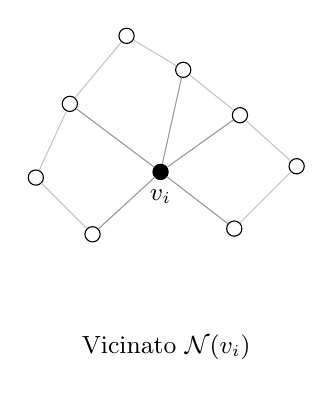
\begin{tikzpicture}[scale=0.72, every node/.style={font=\small}]
    \tikzset{nd/.style={circle, draw, inner sep=0pt, minimum size=5.5pt, fill=white}}
    \node[nd, fill=black, label=below:{$v_i$}] (c) at (2.2,2.1) {};
    \node[nd] (a1) at (0.6,3.3) {};
    \node[nd] (a2) at (1.0,1.0) {};
    \node[nd] (a3) at (3.6,3.1) {};
    \node[nd] (a4) at (3.5,1.1) {};
    \node[nd] (a5) at (2.6,3.9) {};
    \node[nd] (b1) at (0.0,2.0) {};
    \node[nd] (b2) at (4.6,2.2) {};
    \node[nd] (b3) at (1.6,4.5) {};
    \draw[gray!80] (c)--(a1) (c)--(a2) (c)--(a3) (c)--(a4) (c)--(a5);
    \draw[gray!45] (a1)--(b1) (a2)--(b1) (a3)--(b2) (a4)--(b2) (a5)--(b3) (a1)--(b3) (a3)--(a5);
    \node at (2.3,-1.0) {Vicinato $\mathcal{N}(v_i)$};
\end{tikzpicture}
\caption[Vicinato di un nodo su un grafo]{Il vicinato $\mathcal{N}(v_i)$ è un insieme non ordinato e di cardinalità variabile, dipendente dal nodo $v_i$ considerato.}
\label{fig:graph-neighborhood}
\end{figure}

La somma ristretta a $\mathcal{N}(v_i)$ realizza la località; $W^{(l)}$, lo stesso per ogni $i$, realizza la condivisione dei pesi. Quanto all'equivarianza per permutazione, la somma è definita su un insieme di vicini anziché su una sequenza ordinata e dipende da $w_{ij}$ e $h_j^{(l)}$ ma non dagli indici $i,j$ in sé. Rinumerare i nodi permuta di conseguenza $w_{ij}$ e $h_j^{(l)}$, ma lascia $h_i^{(l+1)}$ invariata a parità di nodo fisico~\cite{bronstein2021geometric}.

Si noti che $h_i^{(l+1)}$ non include la rappresentazione precedente del nodo stesso, $h_i^{(l)}$, a meno che $v_i \in \mathcal{N}(v_i)$: la \Cref{sec:gcn-kipf-welling} mostra come la GCN risolva il problema aggiungendo un self-loop a ogni nodo.

\section{La Graph Convolutional Network}
\label{sec:gcn-kipf-welling}

La \cref{sec:from-perceptron-to-graph-layer} ha lasciato aperte due questioni, entrambe implicite nella forma lineare dell'Eq.~\eqref{eq:graph-aggregation}. La prima riprende quanto osservato a chiusura del paragrafo: la somma è ristretta a $\mathcal N(v_i)$, quindi $h_i^{(l+1)}$ non include $h_i^{(l)}$ a meno che $v_i\in\mathcal N(v_i)$ — un nodo, dopo un solo layer, non conserva più alcuna informazione sulla propria rappresentazione precedente. La seconda non è stata ancora discussa: la somma $\sum_j w_{ij}h_j^{(l)}$ non ha alcun vincolo di scala e cresce con il numero e il peso dei vicini di ciascun nodo. Kipf e Welling~\cite{kipf2017gcn} risolvono entrambe le questioni con due correzioni mirate, applicate direttamente alla forma lineare appena derivata, ottenendo la Graph Convolutional Network (GCN).

Si isola momentaneamente la discussione al caso di un solo filtro, con $F_l=F_{l+1}=1$, in cui $W^{(l)}$ si riduce ad uno scalare $\theta$ e $h^{(l)}$ ad un segnale $x\in\mathbb{R}^N$ sui nodi, una restrizione temporanea rimossa successivamente generalizzando a $F$ feature per nodo. Sotto questa restrizione, l'Eq.~\eqref{eq:graph-aggregation} diventa, per ciascun nodo,
$$y_i = \theta\sum_{v_j\in\mathcal N(v_i)}w_{ij}x_j = \theta\,(Wx)_i,$$
ovvero $y=\theta Wx$ in forma matriciale.

La seconda questione riguarda direttamente questo prodotto. $W$ non ha alcun vincolo di scala e un nodo con grado elevato produce una somma di magnitudine maggiore di quella di un nodo periferico, esattamente il problema già incontrato per il Laplaciano nella \cref{sec:graph-laplacian}. Si applica nuovamente la normalizzazione simmetrica $D^{-1/2}(\cdot)D^{-1/2}$ piuttosto che utilizzare la matrice grezza $W$,
$$y = \theta D^{-1/2}WD^{-1/2}x.$$

La prima, invece, è quella lasciata aperta dalla \cref{sec:from-perceptron-to-graph-layer}. La somma normalizzata non include ancora $x_i$, a meno che $v_i$ sia vicino di sé stesso. In caso contrario, il nodo perde ogni contributo diretto della propria rappresentazione. Il modo più diretto per ovviare a questo problema è sommare $x_i$ al risultato, riutilizzando lo stesso $\theta$ già condiviso da ogni vicino invece di introdurre un secondo parametro per il solo termine centrale. Si ottiene così
\begin{equation}
\label{eq:gcn-step3}
y = \theta\left(I + D^{-1/2}WD^{-1/2}\right)x.
\end{equation}

\subsection{Il renormalization trick}

Sottraendo a $2$ lo spettro di $L_{\mathrm{sym}}$, per cui vale $\lambda_{\max}\leq2$~\cite{chung1997spectral}, con uguaglianza se e solo se il grafo ha una componente connessa bipartita\footnote{Un grafo è bipartito se i suoi nodi si dividono in due insiemi e ogni arco collega un nodo del primo a uno del secondo. È un caso non tipico per il grafo di correlazione tra criptovalute di questo studio, dove ogni asset è connesso a molti altri.}, si ottiene lo spettro dell'operatore $I + D^{-1/2}WD^{-1/2}$, contenuto quindi in $[0,2]$. Impilando $l$ layer, l'operatore viene applicato $l$ volte, e le componenti del segnale associate agli autovalori prossimi a $2$ vengono amplificate di un fattore che cresce come $2^l$, con conseguente instabilità numerica e gradienti che esplodono. Kipf e Welling risolvono il problema con il \emph{renormalization trick}. Anziché essere sommato dopo come nell'Eq.~\eqref{eq:gcn-step3}, il self-loop entra nell'adiacenza prima della normalizzazione, ricalcolata sul grafo così modificato,
\begin{equation}
\label{eq:renormalization}
\tilde A = A + I,\qquad \tilde d_{ii}=\sum_j\tilde a_{ij},\qquad \hat A = \tilde D^{-1/2}\tilde A\tilde D^{-1/2},
\end{equation}
dove $A$ denota la matrice di adiacenza, che in questo caso coincide con la matrice $W$ della \cref{def:weighted-graph} essendo il grafo pesato. La sostituzione di $I + D^{-1/2}WD^{-1/2}$ con $\hat A$ non cambia la sostanza dell'operazione (in entrambi i casi ogni nodo combina sé stesso con i propri vicini) ma riporta lo spettro in $[-1,1]$, dove l'applicazione ripetuta non fa crescere l'ampiezza del segnale.

Applicando questa sostituzione e generalizzando l'equazione~\eqref{eq:gcn-step3} da un segnale scalare per nodo a un vettore di $F_l$ feature per nodo — cioè da $x\in\mathbb{R}^N$ a una matrice $H^{(l)}\in\mathbb{R}^{N\times F_l}$ — e da un filtro a $F_{l+1}$ filtri appresi in parallelo, si ottiene infine la regola di propagazione della Graph Convolutional Network (GCN):
\begin{equation}
\label{eq:gcn}
\boxed{\;H^{(l+1)} = \sigma\!\left(\tilde D^{-1/2}\tilde A\tilde D^{-1/2}H^{(l)}W^{(l)} + b^{(l)}\right)\;}
\end{equation}
con $H^{(l)}\in\mathbb{R}^{N\times F_l}$, $W^{(l)}\in\mathbb{R}^{F_l\times F_{l+1}}$, $b^{(l)}\in\mathbb{R}^{F_{l+1}}$ e $\sigma$ non lineare come nell'equazione~\eqref{eq:mlp-layer}, che nell'implementazione dello studio è la ReLU, $\sigma(z)=\max(0,z)$.

\subsection{Lettura della formula}

L'equazione~\eqref{eq:gcn} condensa le correzioni finora discusse.

\begin{description}
    \item[$H^{(l)}$ — Rappresentazioni correnti.] La riga $i$-esima è il vettore di feature del nodo $v_i$ allo strato $l$. Allo strato iniziale $H^{(0)}$ contiene le feature osservate: nel caso del grafo delle criptovalute, sono le grandezze estratte dalla serie storica di ciascun asset (\cref{sec:tc-node-features}).
    \item[$W^{(l)}$ — Trasformazione delle feature.] È una matrice di parametri appresa e condivisa da \emph{tutti} i nodi. Il numero di parametri dipende dalle dimensioni $F_l\times F_{l+1}$ dello spazio delle feature, non da $N$, condivisione dei pesi della \cref{sec:from-perceptron-to-graph-layer}. Un modello addestrato su un grafo può quindi essere applicato ad un grafo con numero diverso di nodi. Si tratta di una proprietà indispensabile per i grafi dinamici della \cref{sec:dynamic-graphs-temporal-question}.
    \item[$\tilde A = A + I$ — Self-loop.] Senza il termine $+I$, l'aggiornamento di un nodo sarebbe funzione dei soli vicini e il nodo perderebbe ad ogni strato la propria informazione: dopo un solo strato la rappresentazione di un asset non conterrebbe più nulla della sua serie storica, ma solo informazioni su quelle delle altre criptovalute. Il self-loop impone che ogni nodo veda anche sé stesso e lo fa senza introdurre un secondo insieme di parametri distinto per il termine centrale.
    \item[$\tilde D^{-1/2}(\cdot)\tilde D^{-1/2}$ — Normalizzazione simmetrica.] Impedisce che i nodi ad alto grado dominino: senza di essa, un nodo connesso a molti altri produrrebbe somme di magnitudine molto maggiore rispetto a nodi periferici, e la rete finirebbe per modellare il grado anziché il segnale. La forma simmetrica $\tilde D^{-1/2}\tilde A\tilde D^{-1/2}$, a differenza della normalizzazione per righe $\tilde D^{-1}\tilde A$, mantiene l'operatore simmetrico e quindi a spettro reale, preservando l'interpretazione spettrale del \Cref{ch:graph-laplacian-theory}. Come già osservato, confina lo spettro in $[-1,1]$ e rende stabile l'impilamento di più strati.
\end{description}

Il coefficiente con cui il nodo $v_j$ contribuisce all'aggiornamento di $v_i$ è dunque $\hat a_{ij} = \tilde a_{ij}/\sqrt{\tilde d_i\tilde d_j}$, con $\tilde d_i = \tilde d_{ii}$, somma pesata in cui il peso decresce con il grado di entrambi gli estremi dell'arco. Questi coefficienti sono \emph{imposti} dalla struttura del grafo e non appresi.

Quanto al costo, l'equazione~\eqref{eq:gcn} si valuta come $\hat A(H^{(l)}W^{(l)})$. La trasformazione delle feature costa $O(NF_lF_{l+1})$ e la propagazione sul grafo, con $\hat A$ in formato sparso, $O(|E|F_{l+1})$. Il costo è dunque lineare nel numero di archi, non quadratico in $N$, a condizione che il grafo sia effettivamente sparso.

La \cref{sec:from-perceptron-to-graph-layer} ha già stabilito che un layer aggrega solo i vicini immediati, la località dell'Eq.~\eqref{eq:graph-aggregation}. In forma matriciale questo si traduce nella struttura di $\hat A$: l'entrata $\hat a_{ij}$ è diversa da zero solo se $(v_i,v_j)\in E$ oppure $i=j$, per costruzione della matrice dei pesi $W$ (\cref{def:weighted-graph}) e del self-loop $\tilde A=A+I$. Il prodotto $(\hat A H^{(l)})_i = \sum_j \hat a_{ij}h_j^{(l)}$ riceve dunque contributo solo dai termini con $j\in\mathcal N(v_i)\cup\{v_i\}$, gli altri sono moltiplicati per zero. Impilando $l$ layer, il campo recettivo si estende a $l$ passi. La GCN ottiene così espressività aumentando la profondità, più strati con pochi parametri ciascuno, invece di allargare il campo recettivo di un singolo strato con più parametri.

\section{Limiti noti delle GNN}
\label{sec:known-limitations-gnn}

Il campo recettivo di una GCN si allarga all'aumentare degli strati impilati. Osservando anche il comportamento delle reti neurali in generale, è naturale aspettarsi che una maggiore profondità porti sempre a una maggiore capacità. In realtà, per i grafi, questa condizione non si verifica.

\subsection{Over-smoothing}
All'aumentare del numero di strati, le rappresentazioni dei nodi tendono a diventare indistinguibili tra loro~\cite{li2018deeper}. Trascurando momentaneamente le non linearità, le trasformazioni $W^{(l)}$ e i bias $b^{(l)}$, impilare $l$ strati GCN equivale ad applicare $\hat A^l$ al segnale di ingresso. Poiché lo spettro di $\hat A$ è contenuto in $[-1,1]$ con autovalore massimo pari a $1$, elevare a potenza schiaccia progressivamente tutte le componenti associate ad autovalori di modulo minore di $1$. Il segnale converge quindi alla proiezione sull'autovettore dominante $\tilde D^{1/2}\mathbf{1}$. Si verifica infatti che $\hat A\tilde D^{1/2}\mathbf1 = \tilde D^{-1/2}\tilde A\mathbf1 = \tilde D^{-1/2}\tilde D\mathbf1 = \tilde D^{1/2}\mathbf1$. È l'analogo, per $\hat A$, di quanto già stabilito nella \cref{prop:zero-multiplicity} per l'autovalore nullo del Laplaciano. Il modo a irregolarità minima non porta informazione strutturale. Questo limite dipende solo dai gradi dei nodi. Le feature di partenza, cioè le differenze tra nodi che il modello dovrebbe sfruttare, non hanno più alcun peso.

\subsection{Grafi densi}
Tutti i vantaggi di costo discussi in questo capitolo sono espressi in funzione di $|E|$ e valgono perché il grafo è sparso. Se $|E|$ si avvicina a $N^2$ il costo $O(|E|F)$ per strato torna quadratico e il vantaggio computazionale svanisce. Su un grafo denso, inoltre, il vicinato a due passi copre già quasi tutti i nodi. L'over-smoothing si manifesta quindi prima, a profondità minore.

Un grafo di correlazione costruito senza filtrare gli archi è per costruzione completo. Il \Cref{ch:dynamic-correlation-graph} affronta la sparsificazione come condizione di funzionamento del modello. Nel grafo di questo studio la soglia calibrata lascia in piedi quasi tutti gli archi, con una densità media di 0,974 che non scende mai sotto 0,733.
La pratica corrente offre una risposta parziale. Le architetture GNN efficaci sui compiti reali usano tipicamente due o tre strati, un campo recettivo modesto che si dimostra preferibile a rappresentazioni più ampie ma rese indistinguibili dall'over-smoothing. La GCN di questo studio applica questa scelta all'estremo inferiore dell'intervallo, con due soli strati e un campo recettivo di due passi, coerente sia con la densità del grafo sia con l'over-smoothing appena discusso.

\section{Baseline}
\label{sec:baselines}

Come termine di paragone per la capacità predittiva della GCN sono state selezionate tre famiglie di modelli che non utilizzano il grafo di correlazione. I modelli naive non guardano le relazioni tra asset o la storia della singola criptovaluta. AR, invece, utilizza esclusivamente la serie storica dell'asset considerato. VAR usa le serie di tutti gli asset senza una struttura esplicita che li leghi.

L'obiettivo di questo confronto è determinare se la struttura relazionale tra criptovalute offre un vantaggio predittivo misurabile rispetto ad un modello che non ne tiene conto. Lo studio tratta questa domanda come una verifica. La baseline di confronto più esigente è quella naive: in finanza la previsione nulla o la media storica battono spesso modelli più sofisticati.

\subsection{Naive}

Un modello naive costituisce un limite inferiore di riferimento per la valutazione di un modello predittivo: non effettua alcuna stima parametrica dai dati, ma restituisce la quantità più elementare disponibile che, nel caso più comune, corrisponde ad un valore costante. La sua funzione non è predittiva in senso proprio, poiché si limita a definire la soglia minima di prestazione che qualunque modello di complessità superiore deve superare per giustificare la propria adozione. Se un modello più sofisticato non supera questo limite, l'apparato aggiuntivo non ha estratto alcuna informazione predittiva utile rispetto al caso banale, indipendentemente dalla sua complessità strutturale.

Nel caso specifico delle serie storiche di rendimenti giornalieri di criptovalute, questa soglia risulta più stringente di quanto intuitivamente atteso. I rendimenti giornalieri presentano una media campionaria statisticamente non distinguibile da zero. Di conseguenza, il predittore naive costante pari a zero si colloca già in prossimità dell'errore quadratico medio (MSE) minimo teoricamente raggiungibile per quella serie. Ne segue che un modello incapace di battere sistematicamente questa baseline non sta catturando alcuna struttura nella media condizionata del processo generatore dei dati, a prescindere dalla qualità del fit osservato in fase di addestramento, che in tal caso è verosimilmente sintomo di overfitting piuttosto che di capacità predittiva reale.

Il progetto implementa due varianti naive. La prima, \texttt{ZeroForecaster}, prevede sempre rendimento nullo per ogni asset,
$$\hat r_{t+1,a} = 0,$$
indipendentemente dall'asset $a$ e dall'origine della previsione $t$.

La seconda, \texttt{HistoricalMeanForecaster}, prevede la media dei rendimenti dell'asset sul blocco di addestramento del fold,
$$\hat r_{t+1,a} = \overline r_a = \frac{1}{T}\sum_{\tau=1}^{T} r_{\tau,a},$$
un valore costante per l'intero periodo di previsione, ricalcolato a ogni fold (intervallo di addestramento e valutazione del protocollo di validazione walk-forward, descritto nella \cref{sec:tc-walkforward}).

\subsection{AR}

Nel caso autoregressivo (AR), la previsione del rendimento futuro si basa esclusivamente sulla storia passata dell'asset. A differenza dei modelli naive, un AR stima dei parametri dai dati di addestramento. Rimane tuttavia un modello univariato, poiché non tiene conto delle relazioni tra le diverse criptovalute.

Il modello autoregressivo di ordine $p$ per l'asset $a$, indicato AR($p$), si scrive
\begin{equation}
\label{eq:ar-model}
\hat r_{t+1,a} = c_a + \sum_{k=1}^{p_a} \phi_{a,k}\, r_{t+1-k,a}.
\end{equation}
Ogni termine $r_{t+1-k,a}$ è il valore osservato $k$ periodi prima dell'origine della previsione, ovvero il $k$-esimo ritardo (\emph{lag}) della serie dei rendimenti dell'asset $a$. L'ordine $p_a$ è il numero di ritardi inclusi nel modello e può differire da un asset all'altro. Il caso $p_a=0$ è degenere: la somma nell'equazione~\eqref{eq:ar-model} è vuota e il modello si riduce alla costante $c_a$, stimata come media campionaria dei rendimenti di addestramento. In questo caso l'AR coincide quindi numericamente con \texttt{HistoricalMeanForecaster}, introdotto nella sottosezione precedente.

I coefficienti $c_a$ e $\phi_{a,k}$ si stimano sui dati della finestra di addestramento del fold con il metodo dei minimi quadrati (Ordinary Least Squares, OLS).

L'ordine $p_a$ non si presta però allo stesso trattamento. Aumentarlo non può mai peggiorare l'adattamento ai dati di addestramento, perché il modello con $p_a$ ritardi è un caso particolare di quello con $p_a+1$ ritardi ottenuto ponendo $\phi_{a,p_a+1}=0$. Minimizzare il solo errore di addestramento porterebbe dunque sempre a preferire l'ordine massimo consentito, indipendentemente dal fatto che i ritardi aggiuntivi catturino una dipendenza reale o solo rumore campionario.

Il Bayesian Information Criterion (BIC) di Schwarz~\cite{schwarz1978estimating} risponde a questa esigenza penalizzando ogni parametro aggiuntivo, oltre alla sola bontà di adattamento,
\begin{equation}
\label{eq:bic}
\mathrm{BIC}(p) = n\ln\hat\sigma_p^2 + (p+1)\ln n,
\end{equation}
ove $n$ è il numero di osservazioni di addestramento e $\hat\sigma_p^2$ l'errore quadratico medio dei residui del modello AR($p$) sullo stesso campione. Confrontando due ordini si preferisce sempre quello a cui corrisponde il valore più basso del criterio: tra $p$ e $p+1$ si sceglie quest'ultimo solo se $\mathrm{BIC}(p+1) < \mathrm{BIC}(p)$. L'ordine $p_a$ adottato è quello che minimizza il BIC su una griglia di candidati compresa tra $0$ e un ritardo massimo $p_{\max}$ fissato in anticipo.

Nel progetto questo schema è implementato dalla classe \texttt{PerAssetARForecaster}, che seleziona l'ordine $p_a$ in modo indipendente per ciascun asset e per ogni fold, poiché l'ordine adeguato ad un asset non è detto lo sia per un altro. Il ritardo massimo ammesso è fissato a $p_{\max}=5$ e la selezione avviene minimizzando il BIC su questa griglia di candidati.

Sui dati di questo studio il BIC seleziona quasi sempre l'ordine nullo: l'ordine medio, calcolato su tutti gli asset e tutti i fold, è pari a $0{,}178$, con l'ordine $0$ scelto nell'85,0\% degli adattamenti. Per la grande maggioranza delle serie il criterio giudica dunque che nessun ritardo della serie stessa migliori la previsione abbastanza da giustificare il parametro aggiuntivo, riducendo l'AR quasi sempre al caso degenere.

\subsection{VAR}
\label{sec:var-baseline}

Rispetto all'AR, il modello a vettori autoregressivi (VAR) lascia che la storia di ogni asset contribuisca alla previsione di tutti gli altri, non solo della propria. Raccogliendo i rendimenti di tutti gli $N$ asset all'istante $t$ nel vettore $r_t\in\mathbb{R}^N$, il VAR di ordine $p$ si scrive
\begin{equation}
\label{eq:var-model}
\hat r_{t+1} = c + \sum_{k=1}^{p} A_k\, r_{t+1-k},
\end{equation}
con $c\in\mathbb{R}^N$ intercetta e $A_k\in\mathbb{R}^{N\times N}$ matrice dei coefficienti del ritardo $k$~\cite{lutkepohl2005new}. La componente $i$-esima dell'equazione~\eqref{eq:var-model} rende esplicito il confronto con l'AR:
$$\hat r_{t+1,i} = c_i + \sum_{k=1}^{p}\sum_{j=1}^{N} (A_k)_{ij}\, r_{t+1-k,j}.$$
Vincolando ogni $A_k$ a essere diagonale, questa espressione si riduce esattamente all'AR dell'equazione~\eqref{eq:ar-model}, applicato separatamente a ciascun asset. L'elemento fuori diagonale $(A_k)_{ij}$, con $i\ne j$, è il canale attraverso cui il ritardo $k$ dell'asset $j$ contribuisce alla previsione dell'asset $i$, canale che nell'AR è assente per costruzione.

Questa generalizzazione ha un prezzo nel numero di parametri: un AR usa $p+1$ parametri per asset, $N(p+1)$ in tutto, mentre un VAR($p$) stima un'intera matrice $N\times N$ per ciascuno dei $p$ ritardi più l'intercetta, per un totale di $N(Np+1)$ parametri. A parità di $p$, il numero di parametri cresce dunque con $N^2$, non con $N$.

La scelta dell'ordine $p$ generalizza quella già vista per l'AR (\cref{eq:bic}), sostituendo la varianza scalare $\hat\sigma_p^2$ con il determinante $|\hat\Sigma_p|$ della matrice di covarianza dei residui stimata sotto il modello di ordine $p$:
$$\mathrm{BIC}(p) = n\ln\left|\hat\Sigma_p\right| + N(Np+1)\ln n.$$
Per $N=1$ le due formule coincidono esattamente, perché il determinante di una matrice $1\times1$ è il suo unico elemento.

Nel progetto la classe \texttt{VARForecaster} implementa due varianti per la scelta dell'ordine. La variante \texttt{var-bic} seleziona $p$ per BIC con lo stesso ritardo massimo $p_{\max}=5$ già usato per l'AR. La variante \texttt{var-p5} fissa invece l'ordine a $p=5$, deciso prima di osservare qualunque risultato sui dati di test, una scelta pre-registrata piuttosto che un valore scelto a posteriori per convenienza.

Sui dati di questo studio le due varianti restituiscono esiti opposti dello stesso compromesso tra adattamento e numero di parametri. Il BIC seleziona $p=0$ su tutti i fold, lo stesso caso degenere già visto per l'AR. Il VAR selezionato non stima alcun coefficiente incrociato e coincide numericamente con la media storica.

Al contrario, \texttt{var-p5} stima $N(Np+1)=15\cdot(15\cdot5+1)=1\,140$ coefficienti a partire da $365$ giorni di addestramento per $15$ asset, ossia $5\,475$ osservazioni complessive: $4{,}80$ per parametro. Ogni parametro aggiunto dà a OLS un grado di libertà in più per ridurre l'errore di addestramento, a prescindere dal fatto che rifletta una dipendenza reale o solo rumore campionario, e questo margine si restringe quanto più i parametri si avvicinano alle osservazioni: con $4{,}80$ per parametro è già minimo. Nel caso limite in cui coincidono, OLS azzera l'errore di addestramento anche su rumore puro, perché esiste sempre una combinazione di coefficienti che passa esattamente per ogni punto osservato. Con \texttt{var-p5} così prossimo a quel regime, molte combinazioni diverse riducono l'errore quasi altrettanto bene, e quella scelta da OLS non si distingue da una che si limita ad assecondare il rumore del campione. Il coefficiente stimato riflette perciò anche il rumore campionario del blocco di addestramento, non solo un'eventuale dipendenza reale: l'adattamento risulta fragile ancora prima di osservarne le prestazioni.
